Bijels require a multiphysics modeling approach to accurately capture the rich array of physical phenomena 
occurring across multiple length and time scales. Within a bijel, one must consider fluid flow, phase separation, particle-fluid coupling, and interparticle 
interactions. The length scales of interest range in the hundreds of nanometer to  tens of micron scale, demanding a model capable of resolving fine structural details while also 
capturing mesoscale dynamics. In the following sections, a comprehensive review of the relevant physical processes is provided, laying the foundation for the 
numerical methods used in this work.

\section{Hydrodynamics}

We begin with a restatement of Reynolds Transport Theorem (RTT) which relates the accumulation of a parameter within a control volume to the difference between the values
of the parameter entering and leaving the volume and the generation and consumption within the volume. The derivation from page 135 to 147 in reference \cite{batchelor_introduction_2000}
is followed. For a non moving and non-deforming volume, the transport equation is given by,

\begin{equation}
    \frac{d}{dt} \int \theta \rho \, dV = \int Q \, dV - \int \theta \rho (\vec{v}_{\text{surf}} \cdot \vec{n}) \, dA
\end{equation}

Where $\theta$ is an intensive quantity of the system such as mass, momentum or energy, $\rho$ is the density of the fluid in the control volume, $Q$ is an effective density
of a source, $V$ is the volume of the control element, $t$ is time, $\vec{v}_{surf}$ is the velocity vector 
of the surface of the volume element and $\vec{n}$ is the surface normal unit vector. \cite{batchelor_introduction_2000} Using the divergence theorem, the expression can be rewritten as

\begin{equation}
    \int \frac{\partial \theta \rho}{\partial t} \, dV = \int Q \, dV - \int \nabla \cdot (\theta \rho \vec{v}_{\text{surf}}) \, dV
\end{equation}

If $\theta = 1$ and $Q = 0$ the continuity equation for fluid density can be written to analyze the mass flux of a control volume given by,

\begin{equation}
    \frac{\partial\rho}{\partial t} + \nabla\cdot\left(\rho\vec{u}\right) = 0
\end{equation}

where $\rho$ is the fluid density and $\vec{u}$ is the fluid velocity. Based on the system being modeled, we assume that the fluid is incompressible, reducing the continuity equation to
$\nabla\cdot \vec{u} = 0$ The momentum conservation equation can also be written by applying Newton's second law to the fluid element. This yields the Cauchy momentum equation, 
where changes in momentum arise due to pressure gradients, viscous stresses, and body forces. The general form of the momentum equation is given by,

\begin{equation}
    \rho \left( \frac{\partial \vec{u}}{\partial t} + (\vec{u}\cdot \nabla \vec{u})  \right) = \nabla \cdot \vec{\vec{\sigma}} + \vec{f}
\end{equation}

where $\vec{f}$ is the force exerted on the fluid from external forces such as gravity and $\vec{\vec{\sigma}}$ is the stress tensor. 
For a Newtonian, isotropic fluid, the stress tensor is given by

\begin{equation}
    \vec{\vec{\sigma}} = -P\mathbb{I} + \eta\left( \nabla \vec{u} + (\nabla \vec{u})^T - \frac{2}{3}(\nabla \cdot \vec{u})\mathbb{I} \right)
\end{equation}

An additional approximation is made that that bulk and dynamic viscosities are related by $\lambda = -\frac{2}{3} \eta$. Substituting this stress tensor into the momentum equation 
and using the relation, $\nabla\cdot \vec{u} = 0$ from the incompressibility constraint, the incompressible Navier-Stokes equation can be derived given by,

\begin{equation}
    \rho \left(\frac{\partial\vec{u}}{\partial t} + (\vec{u}\cdot\nabla)\vec{u} \right) = -\nabla P + \eta \nabla^2 \vec{u} + \vec{f}
\end{equation}

To facilitate numerical simulation and analysis, it is often useful to express the Navier-Stokes equation in non-dimensional form. Introducing characteristic scales for length 
$l_0$, velocity $u_0$, and density $\rho_0$, dimensionless variables are defined as

\begin{equation}
    \bar{l} = \frac{l}{l_0}, \quad \bar{u} = \frac{u}{u_0}, \quad \bar{t} = \frac{u_0 t}{l_0} \quad \bar{\rho} = \frac{\rho}{\rho_0}, \quad \bar{P} = \frac{P}{\rho u^2}, 
\end{equation}

The form of the dimensionless pressure $\bar{P}$ is not unique and depends on whether inertial or viscous effects dominate. The expression shown is 
relevant to an inertial regime. Substituting these into the incompressible Navier-Stokes equation and approximating that no external forces are present 
leads to the dimensionless form:

\begin{equation}
    \frac{\partial \bar{\vec{u}}}{\partial \bar{t}} + (\bar{\vec{u}} \cdot\nabla)\bar{\vec{u}} = \frac{1}{Re} \nabla^2 \bar{\vec{u}} - \nabla\bar{P}
\end{equation}

where the Reynolds number is defined as $Re = \frac{\rho_0 u_0 l_0}{\eta}$ which characterizes the ratio of inertial to viscous forces in the system. For a system
where viscous effects dominate, $Re << 1$ the dimensionless pressure is defined as $\bar{P} = \frac{P l_0}{\eta u_0}$. This yields the alterate form,

\begin{equation}
    Re\left( \frac{\partial \bar{\vec{u}}}{\partial \bar{t}} + (\bar{\vec{u}} \cdot\nabla)\bar{\vec{u}}  \right) = \nabla^2 \bar{\vec{u}} - \nabla\bar{P}
\end{equation}

When substituting the value of $Re$ into the above and approximating the LHS to 0, the Stokes equation is recovered.

\section{Phase separation}

Bijels form through spinodal decomposition of two partially miscible fluids, a process that can be effectively modeled using the Cahn-Hilliard equation. \cite{cahn_spinodal_1961} While the
original equation is written for a concentration of species $c$. For a binary mixture, it can be recast in terms of a conserved scalar order parameter $\phi$, typically representing the 
local concentration difference between the two fluid components. As we are also accounting for the effect of hydrodynamics on the flow of mass, the advection term
from the mass flux $\vec{J}$ cannot be set to 0. Therefore the advective Cahn-Hilliard equation of an incompressible fluid ($\nabla \cdot \vec{v} = 0$) is given by,

\begin{equation}
    \begin{split}
        \nabla \cdot \vec{J} &= \nabla \cdot \phi\vec{u} - M \nabla \mu \\
        \frac{\partial \phi}{\partial t} + \nabla \cdot \vec{J} &= 0 \\
        \frac{\partial \phi}{\partial t} + \vec{u}\cdot\nabla\phi &= \nabla \cdot \left( M \nabla \mu \right)
    \end{split}
\end{equation}

Here, $M$ is the mobility coefficient and $\mu$ is the chemical potential derived from the variation of the free energy functional $F[\phi]$ which is the sum of a bulk free energy
$f(\phi)$ and an interfacial contribution. This formulation allows for the modeling of interfacial tension and the spontaneous formation of bicontinuous domains characteristic of spinodal decomposition.
To capture not only the diffusive separation of phases but also the resulting fluid motion, the Cahn-Hilliard equation is coupled with the Navier-Stokes equation. This is done
through the pressure which is expressed as the sum of the mechanical $P$ and chemical pressure $P_{chem}$ contributions to yield $P_{tot} = P + P_{chem}$. For a binary system, $P_{chem}$ 
can be written as a function of $\phi$ given by,

\begin{equation}
    P_{chem} = \left[ \phi \mu - f(\phi) - \kappa(\phi \nabla^2 \phi + \frac{1}{2}|\nabla \phi |^2 )\right] \mathbb{I} + \kappa \nabla \phi \otimes \nabla \phi
\end{equation}

The divergence of the above expression is found to be $\nabla \cdot P_{chem} = \phi \nabla \mu$. Substituting $P_{tot}$ for $P$ in the Navier Stokes equation,
the Cahn-Hilliard-Navier-Stokes (CHNS) framework is obtained. This coupling is essential in systems like bijels, where advection plays a role in domain 
coarsening. The momentum conservation equation in this framework is given by,

\begin{equation}
    \rho \left(\frac{\partial\vec{u}}{\partial t} + (\vec{u}\cdot\nabla)\vec{u} \right) = \eta \nabla^2 \vec{u} - \nabla P - \phi \nabla \mu
\end{equation}

% Here, $\vec{u}$ is the velocity field, $\rho$ is the fluid density, and $\eta$ is the dynamic viscosity. The term $P_{\text{therm}}$ represents the thermodynamic pressure tensor, which incorporates 
% contributions from gradients in the order parameter and is directly linked to the chemical potential \(\mu\). This tensor encodes the capillary and interfacial forces arising from phase separation 
% and effectively couples the compositional dynamics to the fluid flow.

The CHNS model enables simulation of complex phase-separating fluid systems, capturing both the interfacial evolution and the momentum transfer within the fluid. In the context of bijels, this 
model can be used to predict the formation and stabilization of the bicontinuous structure, especially when interfacial jamming by colloidal particles is introduced.

\section{Implementing the multicomponent Lattice Boltzmann Method} 
\label{section:lbm_hydrodynamics}

The lattice boltzmann method works by evolving a population distribution $f_{i}(\vec{x}, t)$ on a cubic lattice with 
timestep $\Delta t$ with lengthscale $\Delta x$. \cite{qian_lattice_1992, succi_lattice_2018, he_theory_1997} The cubic lattice or stencil is described
DnQm where n and m represent the number of dimensions and directions in the stencil. \cite{succi_lattice_2018, schmieschek_lb3d_2017}
Common stencils include the D1Q5, D2Q9 and D3Q19 stencil, all of which recover mass and momentum conservation and are Galilean invariant.
For energy conservation, a higher order stencil such as D3Q27 is necessary. The D2Q9 and D3Q19 stencils have 9 and 19 populations respectively that include 
connections to nearest and next nearest neighbour points. The D3Q19 
velocity set is used in this work with the indexes $i$ represent each of the 19 velocities and conserves mass and momentum 
to the second order. It can be seen in Figure \ref{fig:d3q19_lattice}. 

\begin{figure}[h]
    \centering
    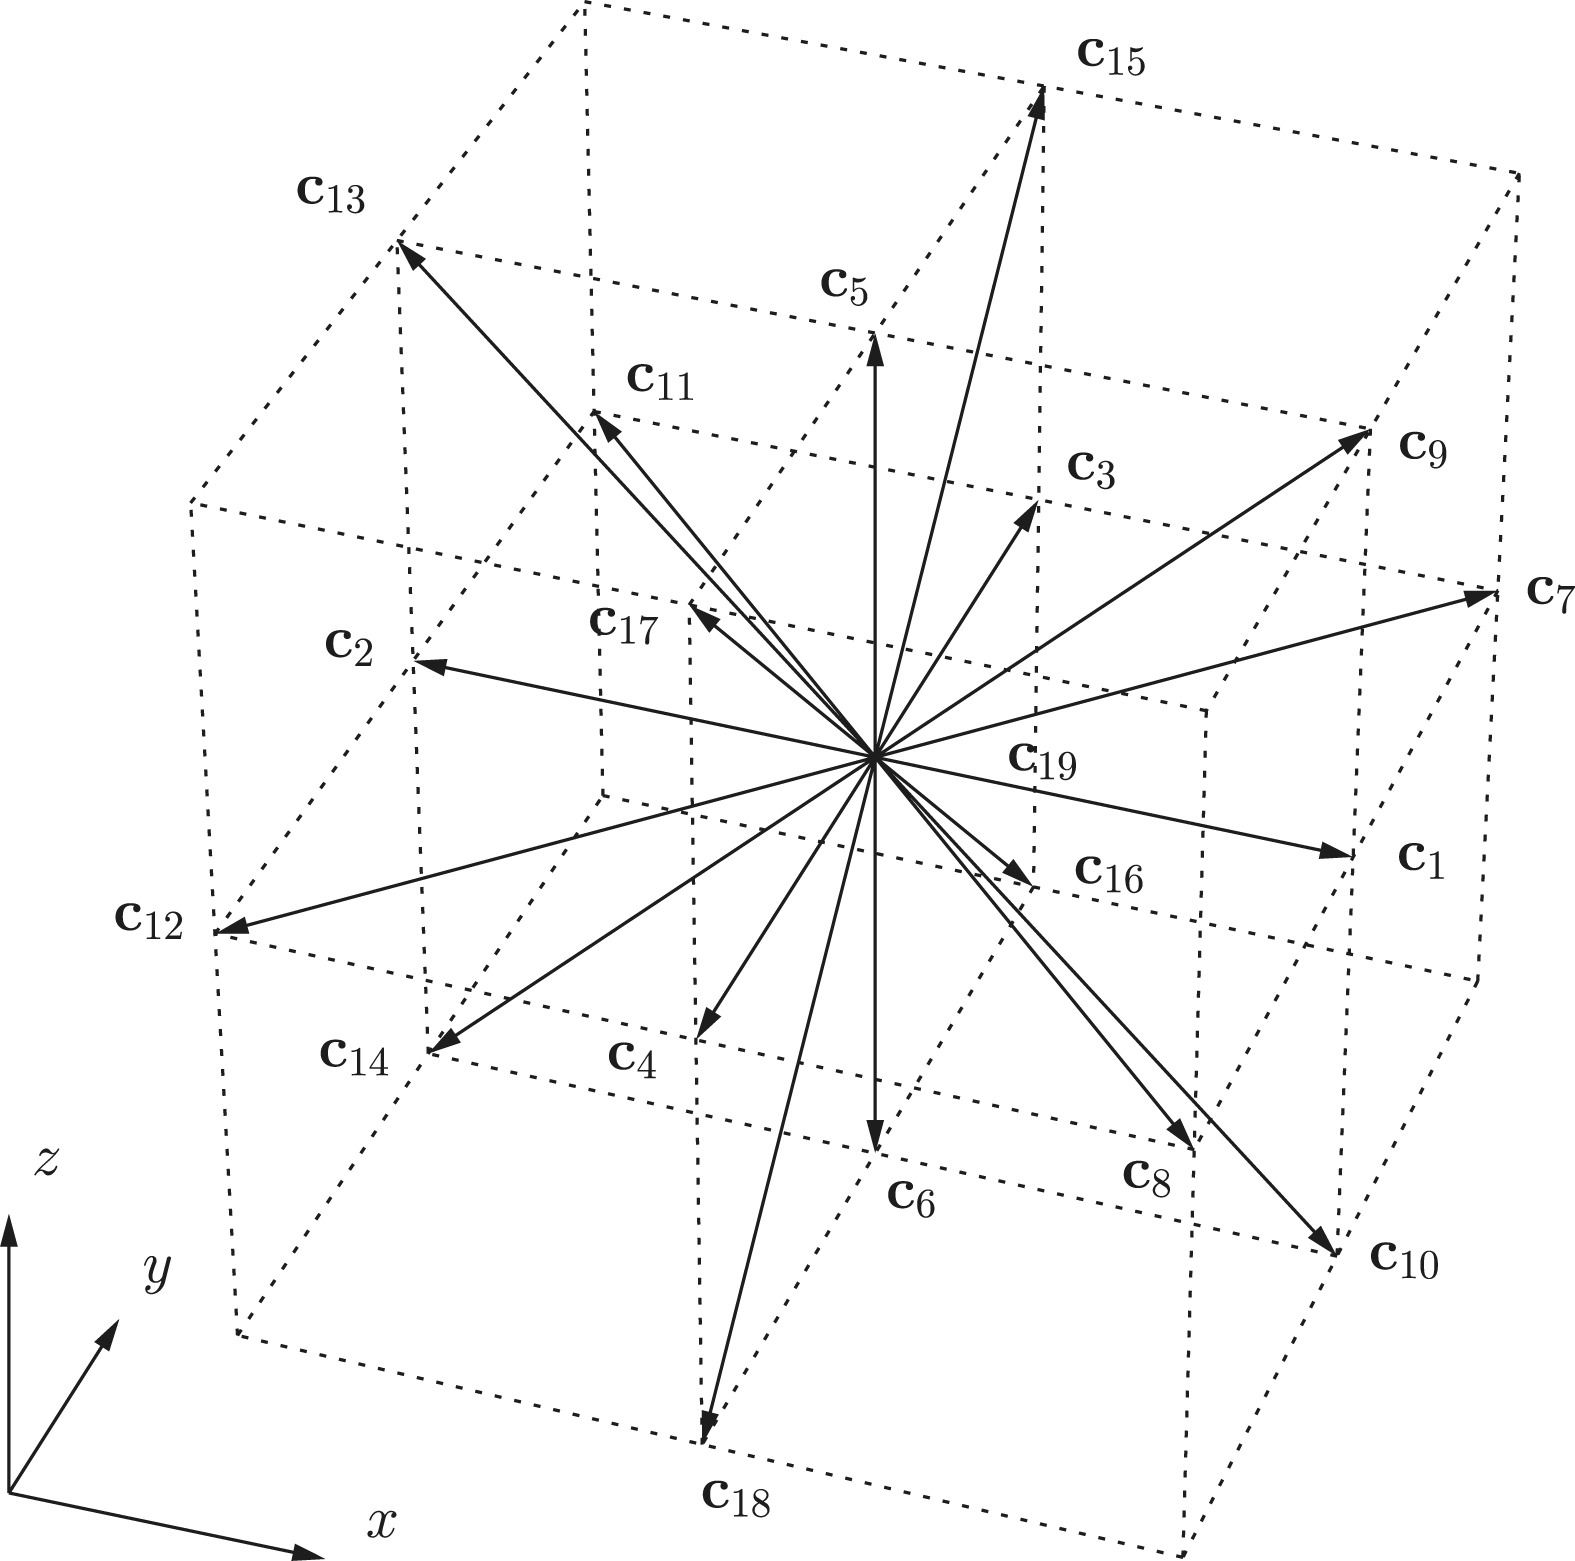
\includegraphics[scale = 1]{figures/methods/d3q19_lattice.jpg}
    \caption{D3Q19 lattice demonstrating the rest, nearest and next nearest direction that correspond to the 19 
    directions $(i)$ of the lattice with lattice velocity $c_{i}$. Reprint of Figure 1 from
    \textit{Schmieschek, S.; Shamardin, L.; Frijters, S.; Krüger, T.; Schiller, U. D.; Harting, J.; Coveney, P. V. LB3D: A Parallel Implementation of the Lattice-Boltzmann Method for Simulation of Interacting Amphiphilic Fluids. Computer Physics Communications 2017, 217, 149-161} 
    with permission from Elsevier under the CC-BY license.}
    \label{fig:d3q19_lattice}
\end{figure}

The LBM is composed of a collision and advection step. In the advection step, the populations at each grid point are propagated to adjacent points in accordance 
with the chosen stencil. During the collision step, the particle population distribution is relaxed towards an equilibrium with a collision operator, at a 
specified relaxation rate. It can take multiple forms depending on the number of
relaxation rates used. The most commonly used variant is the Single Relaxation Time (SRT) operator defined with the Bhatnagar-Gross-Krook (BGK) 
collision operator \cite{bhatnagar_model_1954, qian_lattice_1992}. The BGK model is easy to implement and works well enough in soft matter and
particle-laden flow simulations.

However the BGK operator controls all moments at a single relaxation rate which can induce numerical instabilities and inaccuracies
at higher fluid velocities. \cite{liu_simulation_2023, adhikari_fluctuating_2005} These numerical instabilities can be resolved by using
a Multiple Relaxation Time (MRT) collision operator. However the relaxation rates used in an MRT collision operator must be tuned carefully
to ensure that the appropriate fluid properties are modelled. Simpler variants of the MRT collision operator such as the Two Relaxation Time (TRT)
collision operator have been proposed as a solution that provides some of the benefits of MRT models with the simplicity of SRT models. These 
have facilitated simulation of a wider range of physical phenomena \cite{adhikari_fluctuating_2005, liu_simulation_2023}. The regimes that the simulations 
performed here will take place will be at relatively small Reynolds numbers, mitigating many of the weaknesses of the SRT model while being computatinally
more efficient. Therefore, the SRT collision operator is selected. The combined streaming and 
collision step in LBM, using the BGK operator, is expressed in Equation \ref{eq:LBM_BGK}.

\begin{equation}
    f_{i}(\vec{x} + \vec{c}_{i}\Delta t, t + \Delta t) = f_{i}(\vec{x}, t) - \frac{1}{\tau}(f_{i}(\vec{x}, t) 
    - f_{i}^{eq}(\rho, \vec{u}))
    \label{eq:LBM_BGK}
\end{equation}

The BGK operator limits simulations to low reynolds number and mach numbers to prevent numerical instabilities. 
\cite{qian_lattice_1992} The kinematic viscosity, if using the BGK operator, is obtained from the Chapman-Enskog expansion of \ref{eq:LBM_BGK}
as $\nu = c_s^2(\tau - \frac{\Delta t}{2})$. $c_s$ is the speed of sound of the lattice and is set to $c_s = \frac{1}{\sqrt{3}}$ in the D3Q19 velocity set. 
The equilibrium distribution is obtained from a projection of the 
Maxwell-Boltzmann distribution onto Hermite polynomials. \cite{he_theory_1997, succi_lattice_2018} This is shown in equation 
\ref{eq:LBM_Feq}.

\begin{equation}
    f_i^{\text{eq}}(\rho, \vec{u}) = w_i \rho \left( 1 + \frac{\vec{c}_i \cdot \vec{u}}{c_s^2} + \frac{(\vec{c}_i \otimes \vec{c}_i - c_s^2 \mathbb{I}) : (\vec{u} \otimes \vec{u})}{2c_s^4} \right)
    \label{eq:LBM_Feq}
\end{equation}

where $w_i$ and $\vec{c}_i$ correspond to the weights and lattice velocity vector of each direction in the D3Q19 lattice and $\rho$ and $\vec{u}$ are the fluid density
and velocity at each lattice point. $\rho$ and $\vec{u}$ can be calculated from the zeroth and first moment of the mass distribution $f_i$, given by 

\begin{equation}
    \begin{split}
        \rho &= \sum_i f_i \\
        \rho\vec{u} &= \sum_i f_i \vec{c}_i
    \end{split}
\end{equation}

Using the Chapman-Enskog expansion, the Navier-Stokes equation at the incompressible limit at low Mach
numbers can be recovered. \cite{qian_lattice_1992, he_lattice_1997} The regime accessible through this method is suitable 
for simulations in this work given that $Re < 100$ and $Ma < 0.01$, fulfilling the stability 
criterion and usage requirements for the presented hydrodynamic model.
The momentum flux tensor is calculated from the Chapman-Enskog expansion of \ref{eq:LBM_BGK} to the second order yielding,

\begin{equation}
    \begin{split}
        \rho\frac{\partial \vec{u}}{\partial t} + \nabla \cdot \Pi &= 0 \\
    \end{split}
\end{equation}

The momentum flux tensor can be expressed as a sum of the equilibrium and non-equilibrium components of the stress tensor, denoted by 0 and 1 respectively given by,

\begin{equation}
    \begin{split}
        \Pi^{(0)} &= \sum_i f_i^{eq} \vec{c}_i \otimes \vec{c}_i = p\mathbb{I} + \rho \vec{u} \otimes \vec{u} \\
        \Pi^{(1)} &= (1 - \frac{1}{2 \tau})\sum_i f_i^{neq} \vec{c}_i \otimes \vec{c}_i = -\eta (\nabla \vec{u} + (\nabla \vec{u})^T)
    \end{split}
\end{equation}

With $p = \rho c_s^2$.

\subsection{Non-ideal mixing}
\label{section:lbm_non_ideal_mixing}

The SC model mimics Cahn-Hilliard type behaviour through a force applied from the other fluid species $k'$ in adjacent 
cells $\vec{x'}$ on fluid species $k$ at point $\vec{x}$. \cite{shan_lattice_1993, shan_simulation_1994, 
shan_multicomponent_1995, he_discrete_1998, jansen_bijels_2011, chin_lattice_2002} Both fluid species are defined
by their own distribution equation defined in Equation \ref{eq:LBM_BGK} The strength of this force is controlled 
through an interaction parameter, $g_{kk'}$ with no contribution from self interaction of the fluid as these are 
set to zero. The SC force can then be written out in Equation \ref{eq:sc_model}.

\begin{equation}
\vec{F}_k(\vec{x}) \Delta t = - \sum_{k'} \sum_i \frac{w_i}{c_s^2} g_{kk'} \psi_k(\vec{x})\psi_{k'}(\vec{x}+\vec{c}_i) \vec{c}_i
\label{eq:sc_model}
\end{equation}

An effective mass of each fluid at node $\vec{x}$ is used in place of the density to scale it between zero 
and one and is defined as $\psi^{k}(\vec{x},t) = \rho_{0}\left[1 - \exp(-\frac{\rho^{k}(\vec{x}, t)}{\rho_{0}})\right]$ where
$\rho_0$ is the reference density and is set to $\rho_0 = 1 \frac{\Delta m}{\Delta x^3}$. 
In this model, the SC force is incorporated into the macroscopic velocities that are then used to calculate the equilibrium
distribution $f_{i}^{k, eq}$ for fluid $k$, defined as,

\begin{equation}
\vec{u}_k^{\text{eq}} = \vec{u}' + \frac{\tau_k}{\rho_k} \vec{F}_k
\end{equation}

Where $\vec{u}'$ is defined as the common grid velocity and is calculated from $f_i^k$ below

\begin{equation}
    \sum_k \frac{\rho_k}{\tau_k} \vec{u}' = \sum_k \frac{1}{\tau_k}\sum_i f_i^k\vec{c}_i
\end{equation}

This recasting of the velocity ensures that in the absence of forces, the total momentum of the system is conserved. 

% \textcolor{blue}{https://doi.org/10.1103/PhysRevE.84.046710}

\subsection{Suspended particle dynamics}
\label{section:lbm_colloids}

Suspended particles will be coupled to the LB fluid based on the work conducted by Ladd. \cite{ladd_numerical_1994, 
aidun_direct_1998, ladd_lattice-boltzmann_2001} The particles follow Newtonian mechanics with the particle force and
rotational inertia defined using differential equations

\begin{equation}
    \begin{split}
    \vec{F_p} = m_p \frac{d \vec{u}_p}{dt} , \\
    \vec{D_p} = \vec{J}_p \frac{d \vec{\omega}_p}{dt} ,
    \label{eq:md}
    \end{split}
\end{equation}

$\vec{F_p}$ and $\vec{D_p}$ represent the force and torque acting on a particle with mass $m_p$ and moment of inertia 
$\vec{J}_p$. $\vec{u}_p$ and $\vec{\omega_{p}}$ are the linear and angular velocities of the particle. The equations of 
motion are evolved over time using a leapfrog integrator. \cite{jansen_bijels_2011}

The particles are discretized on the lattice according to the method laid out in Ladd 1994 and Aidun 1998
\cite{ladd_numerical_1994,aidun_direct_1998}. Nodes representing the particle are marked as solid nodes that replicate
a no-slip boundary condition through a moving bounce-back boundary. This is implemented into the distribution function
by reflecting the outgoing populations of $f_i^k$ to the opposite lattice velocity $f^k_{i^\star}$ given by

\begin{equation}
    f^k_{i^\star}(\vec{x}, t+\Delta t) = f^{k,\star}_i(\vec{x}, t) - \frac{2w_i}{c_s^2} \rho \vec{u}_i \cdot \vec{c}_i ,
\end{equation}

where $\vec{u}_i = \vec{u}_p + \vec{omega}\times \vec{r_i}$ which represents the difference between the particle velocity and the 
velocity of the particle surface. The location of the particle surface $r_i$ is calculated as $r_i = \vec{x} + \frac{\Delta t}{2}\vec{c}_i - \vec{x}_{cm}$ 
where $\vec{x}_{cm}$ is the center of mass of the particle.
This facilitates momentum exchange between particle and fluid which can be calculated analytically as 
\(\Delta\vec{p}^k_i = 2 f^{k,\star}_i(\vec{x},t)\vec{c}_i - \frac{2w_i}{c_s^2}\rho(\vec{u}_i\cdot\vec{c}_i)\vec{c}_i\).
The sum of the momentum change across the surface of the particle is computed to obtain the force and torque on the particle,

\begin{equation}
    \begin{split}
    \vec{F}_p &= \sum_{k,i} \frac{\Delta \vec{p}^k_i}{\Delta t} , \\
    \vec{T}_p &= \sum_{k,i} \frac{\Delta\vec{p}^k_i}{\Delta t} \times \vec{r}_i .
    \end{split}
\end{equation}

As the particle moves, the nodes representing the particle are updated, with newly covered grid points marked as solid and 
uncovered nodes marked as fluid. When a grid point is covered, the momentum contained in that lattice point is added to the 
total force of the particle,

\begin{equation}
    \vec{F}_p = -\sum_{k,i} f_i^k(\vec{x},t)\vec{c}_i .
\end{equation}

Upon uncovering of a grid point, it is assigned a density value that represents the average of all adjacent fluid sites,

\begin{equation}
    \rho^k(\vec{x},t) = \frac{1}{N_{\text{f}}} \sum_{i_{\text{f}}} \rho^k(\vec{x}+\vec{c}_{i_{\text{f}}n}, t)
    \label{eq:fill_particles}
\end{equation}

where $N_{\text{f}}$ is the number of fluid nodes around the uncovered node and $\vec{c}_{i_{\text{f}}n}$ is the lattice velocity 
in the uncovered grid point that points to a surrounding fluid node.

\subsection{Particles near contact}
\label{section:particles_near_contact}

For particles close to contact, meaning with inter-surface distances under 1 lattice unit the hydrodynamics are unresolved as the
distance is smaller than what the model can resolve. Lubrication forces are added to reduce the likelihood of particle overlap. For 
spherical particles, this is defined in Equation \eqref{eq:lubrication}

\begin{equation}
    \vec{F}_l = -6 \pi \eta \frac{R_1^2 R_2^2}{\left(R_1+R_2\right)^2}\left(\frac{1}{|\vec{r}_{ij}|-R_1-R_2}-\frac{1}{d_c}\right) \frac{\left(\vec{u}_{12}\cdot\vec{r}_{12}\right)\vec{r}_{12}}{|\vec{r}_{12}|^2} ,% \qquad d<d_c,
    \label{eq:lubrication}
\end{equation}

where $R_i$ and $R_j$ are the radii of each particle involved in the interaction, $\vec{r}_{ij}$ is the distance
vector between the particle centers, $\vec{u}_{ij}$ are the relative velocities of the particles and $d_c$ 
is the cutoff distance when the lubrication force begins to act. If particles are able to overcome the lubrication forces, 
a hertzian contact force is also added to ensure that there is no particle overlap, defined in Equation \eqref{eq:hertz}

\begin{equation}
    \phi_{H} = K_{H}(R_i + R_j - |\vec{r}_{ij}|)^{5/2}, r < R_i + R_j
    \label{eq:hertz}
\end{equation}

$K_H$ is the force constant used to push particles apart. 

\subsection{Ellipsoidal_particles}
\label{section:ellipsoidal_particles}

To correct for the ellipsoidal particles used in this work, 
the formulas presented in Eqs \ref{eq:lubrication} and \ref{eq:hertz} can be generalized using the route followed 
in Gunther et al. and Davies et al., inspired by Berne and Pechukas. \cite{gunther_timescales_2014, davies_interface_2014} 
They first begin by rewriting the lubrication and Hertzian contact forces as a function of the particle orientation and 
aspect ratio of the particles.

\begin{equation}
    \begin{split}
    \phi(\vec{r}_{ij}) &= {\epsilon} \tilde{\phi}\left(\frac{\vec{r}_{ij}}{{\gamma}}\right) , \\
    \vec{F}(\vec{r}_{ij}) &= {\epsilon} \tilde{\vec{F}}\left(\frac{\vec{r}_{ij}}{{\gamma}}\right) .
    \end{split}
\end{equation}

For the lubrication force \eqref{eq:lubrication}, we choose
${\gamma}=R_1+R_2$ and ${\epsilon}=\frac{6\pi\eta R_1^2 R_2^2}{{\gamma^3}}$, and for the
Hertz potential we chose ${\gamma}=R_1+R_2$ and ${\epsilon}=K_H\gamma^{5/2}$. For two identical, rotationally
symmetric ellipsoidal particles with unit orientation vectors $\hat{\vec{o}}_i$ and $\hat{\vec{o}}_j$, we then replace $\epsilon$ and $\gamma$ by
the functions

\begin{equation}
    \begin{split}
    \tilde\epsilon\left(\hat{\vec{o}}_i, \hat{\vec{o}}_j\right) &= \frac{{\epsilon}}{\sqrt{1-\chi^2}} , \\
    %\qquad \chi = \frac{\left(\alpha^2-1\right)R_\parallel^2}{\left(\alpha^2+1\right)R_\parallel^2}\left(\hat{\vec{o}}_i\hat{\vec{o}}_j\right) , \\
    \tilde\gamma\left(\vec{r}_{ij}, \hat{\vec{o}}_i, \hat{\vec{o}}_j\right) &= \frac{{\gamma}}{\sqrt{1-\frac{\chi}{2}\left[ \frac{\left(\hat{\vec{r}}_{ij}\cdot\hat{\vec{o}}_i+\hat{\vec{r}}_{ij}\cdot\hat{\vec{o}}_j\right)^2}{1+\chi\left(\hat{\vec{o}}_i\hat{\vec{o}}_j\right)} + \frac{\left(\hat{\vec{r}}_{ij}\cdot\hat{\vec{o}}_i-\hat{\vec{r}}_{ij}\cdot\hat{\vec{o}}_j\right)^2}{1-\chi\left(\hat{\vec{o}}_i\hat{\vec{o}}_j\right)} \right] }} , \\
    \chi &= \frac{\alpha^2-1}{\alpha^2+1} , \\
    \end{split}
\end{equation}

where $R_{\parallel}$ is the particle radius along the
symmetry axis and $\alpha=\frac{R_{\parallel}}{R_{\perp}}$ the aspect
ratio of the particle. The anisotropic Hertz potential and lubrication
force are then defined as
%
\begin{equation}
    \begin{split}
    \phi\left(\vec{r}_{ij}, \hat{\vec{o}}_i, \hat{\vec{o}}_j\right) &= \epsilon\left(\hat{\vec{o}}_i, \hat{\vec{o}}_j\right) \tilde{\phi}\left(\frac{\vec{r}_{ij}}{\gamma\left(\vec{r}_{ij}, \hat{\vec{o}}_i, \hat{\vec{o}}_j\right)} \right) , \\
    \vec{F}\left(\vec{r}_{ij}, \hat{\vec{o}}_i, \hat{\vec{o}}_j\right) &= \epsilon\left(\hat{\vec{o}}_i, \hat{\vec{o}}_j\right) \tilde{\vec{F}}\left(\frac{\vec{r}_{ij}}{\gamma\left(\vec{r}_{ij}, \hat{\vec{o}}_i, \hat{\vec{o}}_j\right)} \right) .
    \end{split}
\end{equation}

\subsection{Magnetic field and particle coupling}
\label{section:lbm_colloids_magnetics}

The magnetic dipole potential is defined as

\begin{equation}
    U_{ij} = \frac{\mu_0 m_i m_j}{4\pi |r_{ij}|^{3}} \left[ \Hat{\vec{o_i}}\cdot \Hat{\vec{o_j}} - 
    3(\Hat{\vec{o_i}} \cdot \Hat{\vec{r_{ij}}})(\Hat{\vec{o_j}} \cdot \Hat{\vec{r_{ij}}}) \right]
    \label{eq:magnet_potential}
\end{equation}

Where $\mu_0 = 4\pi \cdot 10^{-7} \frac{H}{m}$,  $\Hat{\vec{o_i}}$ is the orientation unit vector of particle 
$i$, $\Hat{\vec{r_{ij}}}$ is the unit distance vector between particles $i$ and $j$ and $m_i$ is the magnitude the 
magnetic dipole of particle $i$. From the potential, the force and torque of the dipole force between particles 
can be found. These expressions are shown in equations \ref{eq:dipole_magnetic_force} and \ref{eq:dipole_magnetic_torque} 
for the force and torque respectively.

\begin{equation}
    \vec{F}_{ij} = \frac{3 \mu_0 m_i m_j}{4 \pi} \left[ \frac{5( \Hat{\vec{o_i}} \cdot \Hat{\vec{r_{ij}}} )(\Hat{\vec{o_j}}
    \cdot \Hat{\vec{r_{ij}}})}{|\vec{r_{ij}}^4|}\Hat{\vec{r_{ij}}} - \frac{(\Hat{\vec{o_i}} \cdot \Hat{\vec{o_j}})\Hat{\vec{r_{ij}}} + 
    (\Hat{\vec{o_i}} \cdot \Hat{\vec{r_{ij}}})\Hat{\vec{o_j}} + (\Hat{\vec{o_j}} \cdot \Hat{\vec{r_{ij}}})\Hat{\vec{o_j}} }{|\vec{r_{ij}}|^4} \right]
\label{eq:dipole_magnetic_force}
\end{equation}

\begin{equation}
    \vec{T}_{ij} = \frac{\mu_0 m_i m_j}{4 \pi}\left[ \frac{3(\Hat{\vec{o_j}} \cdot \Hat{\vec{r_{ij}}})\Hat{\vec{o_i}} \times \Hat{\vec{r_{ij}}} }
    {|\vec{r}_{ij}|^3} - \frac{\Hat{\vec{o_i}} \cdot \Hat{\vec{o_j}} }{|\vec{r}_{ij}|^3}\right]
    \label{eq:dipole_magnetic_torque}
\end{equation}

Equations \ref{eq:magnet_force} and \ref{eq:magnet_torque} are used to calculate the force and torque that the 
field exerts on each particle.

\begin{equation}
    \vec{F}_{j} = m_j(\Hat{\vec{o_j}} \cdot \nabla \vec{B}_{i})
    \label{eq:magnet_force}
\end{equation}

\begin{equation}
    \vec{T}_{j} = m_j(\Hat{\vec{o_j}} \times \vec{B}_{i})
    \label{eq:magnet_torque}
\end{equation}

The total force and torque exerted on each particle is the sum of the particle dipole interaction and the field 
dependent contribution. 

\section{Simulation setup}
\label{section:sim_setup}

Critical parameters in this system include fluid density $\rho_f$, dynamic viscosity $\eta$, surface tension $\sigma$, 
length scale $L$, and applied magnetic field strength $B$. The dynamic viscosity and surface tension is determined 
by the relaxation time using the BGK collision operator, $\eta = \rho_f c_s^2(\tau - \frac{1}{2})$ and $g_{kk'}$ 
respectively. Dimensionless numbers derived from the Buckingham Pi theorem are the Reynolds number
($Re = \frac{\rho u L}{\eta}$), Weber number ($We = \frac{\rho u^2 L}{\sigma}$), and magnetic bond number 
($\Bar{B} = \frac{Bd}{\sigma A}$). Here, $u$ is velocity, $d$ is the particle's dipole moment, and $A$ is the 
particle's cross-sectional area. The system's velocity and length scale are set as the domain size and coarsening rate. 
Parameters for the fluid, particle, and non-ideal mixing model used in the simulations are summarized in Table 
\ref{table:model_params}.

\begin{table}
    \centering
    \caption{Summary of the parameters corresponding to the fluid, particle and model used in the simulations. 
             LB parameters can be converted to their real world equivalents using the unit conversions provided.}
    \label{table:model_params}
    \begin{tabular}{|c|c|}
    \hline
    Parameter & Value \\ [0.5ex] 
    \hline\hline
    $L_x$ & 256 $\Delta x$ \\
    $\rho_f$ & 0.7 $ \frac{\Delta m}{(\Delta x)^3}$\\
    $\nu_f$ & 1/6 $\frac{\Delta x}{(\Delta t)^2}$ \\
    $\sigma $ & 0.0267 $\frac{\Delta m}{(\Delta t)^2}$ \\
    $\tau$ & 1 $\Delta t$\\
    $g_{kk'}$ & 0.08 $\frac{(\Delta x)^5}{\Delta m(\Delta t)^2}$\\
    $\phi_f$ & 0.5 \\
    $\phi_p$ & 0.15 \\
    $n_p$ & 1200 \\
    $\rho_p$ & 1 $ \frac{\Delta m}{(\Delta x)^3}$\\
    $V_p$ & $2000\pi/3 (\Delta x)^3$ \\
    $m$ & 1 $\frac{\Delta q}{\Delta t(\Delta x)^2}$\\
    $d_c$ & 2/3 $\Delta x$ \\
    $K_H$ & 100 $\frac{\Delta m}{(\Delta x)^{1/2}(\Delta t)^2} $\\
    \hline
    \end{tabular}
\end{table}


In these simulations, the aspect ratio is defined as $\alpha = \frac{R_{\parallel}}{R_{\perp}}$ with $\alpha = 0.5, 1, 2$ 
used in these simulations. All particle geometries are volume matched, based on the spherical particle volume. For the 
spherical particle, the radius was set at $R_{\parallel} = R_{\perp} = 7.9 \Delta x$ which sets the $\alpha = 0.5$ particles to 
$R_{\parallel} = 5 \Delta x, R_{\perp} = 10 \Delta x$ and the $\alpha = 2$ particles to $R_{\parallel} = 12.6 \Delta x, R_{\perp} = 6.3 \Delta x$. 
$R_{\parallel}$ and $R_{\perp}$ is the radius of the particle parallel and perpendicular to the symmetry axis of 
the particle respectively. These values are identical to what was used in Gunther et al, allowing comparisons to the 
trends they observed. \cite{gunther_timescales_2014} The particles were randomly placed in the system and an equilibration
step was performed to push the particles further away from each after placement. Once equilibration is performed, a 
constant magnetic field is switched on with dimensionless strengths defined using $\bar{B}$.

The initial condition of the system when simulating bijels sets the density of each grid to $0.5\rho_f + \varepsilon$ of 
each fluid where $\varepsilon = 0.0001N(0,1)$. The model parameters trigger phase separation with a sharp interface at 
the start of the simulation. Periodic boundary conditions are applied on all sides unless the system is undergoing shear. 
The shear gradient is applied as a velocity in the z direction across the x axis and implemented as a Lees-Edwards 
(LE) boundary condition in the yz planes. \cite{wagner_leesedwards_2002, lorenz_lees-edwards_2009, yang_capillary_2022} 
These boundaries move with velocities $u_{LE}$ and $-u_{LE}$ to conserve momentum, with a shear rate 
$\dot{\gamma} = \frac{2 u_{LE}}{L_x}$. LE boundaries are preferred over walls to avoid affecting viscosity measurements. 
\cite{wagner_leesedwards_2002, lorenz_lees-edwards_2009, yang_capillary_2022}

Bijel templates have been synthesized using water/2-6-lutidine for further applications. \cite{lee_making_2013} 
While intrinsically polymerizable bijels have been prepared using oligomeric polymers, STRIPS and VIPS currently 
utilize small molecule liquids in their bijel casting mixtures. Therefore, an experimentally viable system using 
water/2-6-lutidine will be discussed in the context of the work presented here. The critical temperature (UCST) 
for this system is $T_c = 34 ^{\circ}\text{C}$, with many systems heated to $T = 40^{\circ}\text{C}$ to form the bijel. At this 
temperature, the fluid properties are $\sigma = 0.22 \text{mN/m}$ and $\eta = 2.38 \text{mPas}$. \cite{grattoni_lower_1993} 
Fei et al. developed a method to synthesize polystyrene microparticles ($R_p = 2\,\mu\text{m}$) with tunable geometries 
by mechanically stretching or compressing them, then coating them with nickel to create magnetic microparticles with 
a dipole moment of approximately$\approx 3 \cdot 10^{-14} \text{Am}^2$. \cite{fei_active_2017, fei_magneto-capillary_2020} 
Comparing the physical properties to simulation parameters, the simulations correspond to a length scale of
$\Delta x = 252 \cdot 10^{-9} \text{m}$, timescale of $\Delta t = 624 \cdot 10^{-9} \text{s}$, 
mass scale of $\Delta m = 2.24 \cdot 10^{-15} \text{kg}$ and charge scale of $\Delta q = 2.948 \cdot 10^{-7} \text{C}$. 

\section{Model results}
\label{section:model_results}

\subsection{Surface tension}
\label{section:model_surface_tension}

In experiments, Wilhelmy and ring tensionometry are used to measure the surface tension from the force needed 
to break through the interface. Pendant drop tensionometry is also used by measuring the pressure required to 
maintain a droplet of analyte at a various sizes and utilizing the Young-Laplace equation to calculate the 
surface tension of the system. \cite{sun_assembly_2013, berry_measurement_2015}
Upon extrusion of a droplet from a reservoir, the size of a droplet is determined by the balance between 
cohesive forces between bubble molecules and geometrical forces that attempt to reduce the curvature of a 
system by increasing its size. For spherical droplets, the equation simplifies to 
$\Delta P = \frac{2 \sigma}{R_d}$ where $\Delta P$ is the difference in scalar pressure 
between the center of the droplet and the ambient pressure, $\sigma$ is the surface tension 
of the interface and $R_d$ is the radius of the droplet. 

\begin{figure}[h]
    \centering
    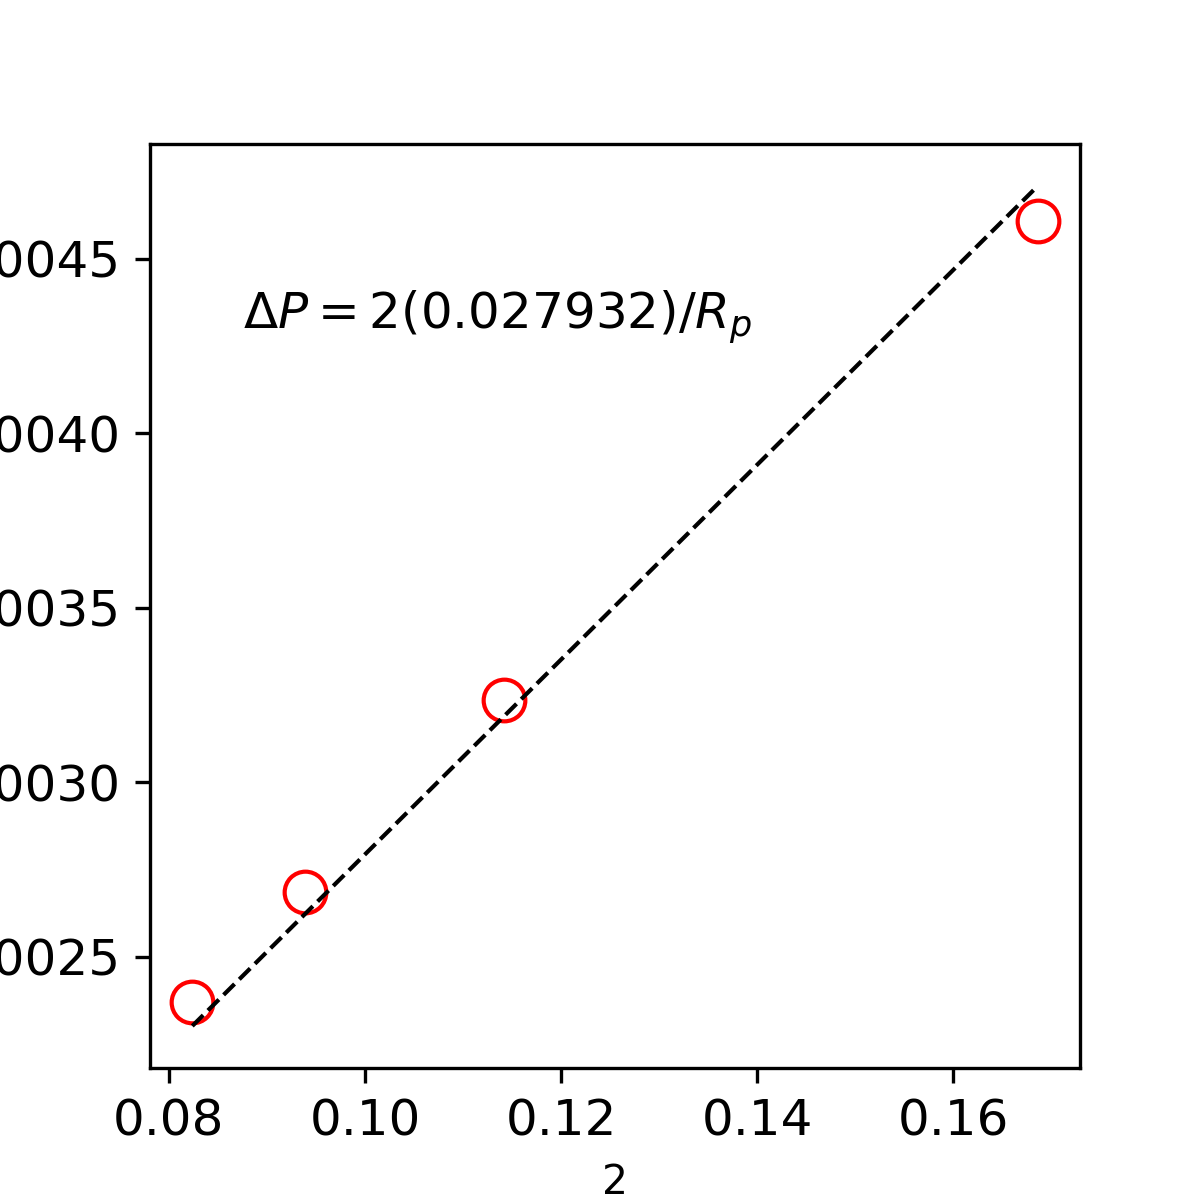
\includegraphics[scale = 0.5]{figures/model_validation/surface_tension.png}
    \caption{Plot of the surface tension of the multicomponent model in this work calculated using the 
    Young-Laplace equation.}
    \label{fig:young_laplace_valid}
\end{figure}

Using the fluid and non-ideal mixing parameters defined in Table \ref{table:model_params}, a single water in oil 
droplet, was initialized in the center of the system and run till the droplet radii reached steady state. 
This process was repeated for various droplet diameters, specified between 70 and 85 \% of the system size at 5\% 
increments. The system had a box length of $L = 64 \Delta x$ and was run for $50000 \Delta t$ timesteps with periodic boundary conditions 
on all sides. Data was saved every 10000 timesteps with only the last timestep used to calculate the values shown. Due 
to the diffuse interface present in this method, the density profiles were verified to be at steady state at the end of 
the simulation before further analysis was performed. \cite{frijters_effects_2012} Past work also showed that the 
pressures remained constant after 5 lattice units away from the interface. \cite{frijters_effects_2012} 

The pressure difference was calculated using the difference in scalar pressure between the center of the droplet and 
one of the corners of the box. Two techniques exist to calculate the radius of the droplet. The first directly measures 
the distance between opposite points of the droplet as measured from the density profile at opposite points of the droplet, 
and the second is based upon the total mass and density of the fluid making up the droplet. The second method offers greater 
accuracy by avoiding discretization errors that may exist in the first method, and also allows for the correction of 
particle volume at the interface if the system contained them. First, a local effective mass density 
$\rho^b_{eff} = \rho^{b}_{d} - \rho^{b}_{m}$ is found by calculating the difference in density between the blue 
fluid in the droplet and in the matrix. Next, the droplet mass is calculated as $M_d = \sum_{\vec{x}}{\rho_{eff}^{b}}$. 
The radius of the droplet can then be calculated from the mass and density of the droplets as $R_d = \sqrt[3]{\frac{3}{4\pi} 
\frac{M_d}{\rho^b_d - \rho^b_m}}$. To linearize the plot, the $\Delta P$ was plotted against $\frac{2}{R_d}$ with 
$\sigma$ being the slope of the fit.

Figure \ref{fig:young_laplace_valid} shows the results of the fit conducted of the Young-Laplace equation demonstrating 
that under these fluid and mixing parameters, the surface tension is $\sigma = 0.0267$. The fit was performed using 
\texttt{scipy.optimize.curve\_fit} with the fit function defined as $y = mx$.